% ----------------------------------------

\subsection{Problem}

% ----------------------------------------

\begin{frame}

\frametitle{Scenario}
\framesubtitle{Hypotesis}

In this scenario the only uncertain parameters are the \textbf{graph weights}.

Alongside the other operations, the learner will run a \textbf{graph estimation} algorithm to build an accurate representation of the graph at each time step.

Meanwhile, since the \textbf{$\alpha$-functions} are known, there is no need to estimate them and they can be applied directly in the optimization problem.

\end{frame}

% ----------------------------------------

\subsection{Implementation}

% ----------------------------------------

\begin{frame}

\frametitle{Solving the problem}
\framesubtitle{Prediction}

Since there is no need to estimate the $\alpha$-functions, the best allocation is calculated using the \texttt{find\_optimal\_superarm} function used to obtain thebest estimation when the $\alpha$-functions are known.

The only difference is that a custom graph needs to be specified since we don't have access to the real graph weights.

\end{frame}

% ----------------------------------------

\begin{frame}

\frametitle{Graph estimation}

The learner contains a graph representation that is updated at each time step; the graph representation is not updated directly but through a function called \texttt{graph\_estimate}, which collects samples from various \textbf{beta distributions} for each graph weight deleting \textit{self-loops} and non-existent edges.

The parameters of the \textbf{beta distributions} ($\alpha$ and $\beta$) are defined for each edge of the graph and represent the effective quantities that are updated whenever the function \texttt{learn} is called on the learner.

\end{frame}

% ----------------------------------------

\begin{frame}

\frametitle{Parameters update}

Whenever we want to make the \textbf{graphless learner} learn by calling its dedicated function, the learner analyzes all of the interactions given as a parameter and looks at the path that the users traversed by comparing it with the current graph representation.

If a certain edge is taken or not by a given user, the $\alpha$ and $\beta$ parameters are updated accordingly.

When \texttt{predict} is called again, the graph representation is then generated from scratch by drawing samples from the \textbf{beta distributions} with the updated parameters.

\end{frame}

% ----------------------------------------

\subsection{Results}

% ----------------------------------------

\begin{frame}[plain]

\frametitle{Reward and regret}
\framesubtitle{Graphless}

\begin{center}
	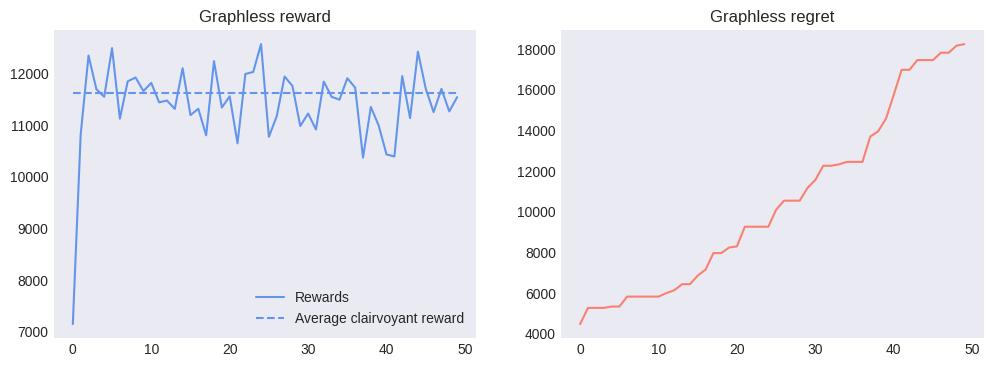
\includegraphics[scale=0.4]{img/Graphs/graphless/image1.png}
\end{center}

\end{frame}

% ----------------------------------------

\begin{frame}[plain]

\frametitle{Average reward and regret}
\framesubtitle{Graphless}

\begin{center}
	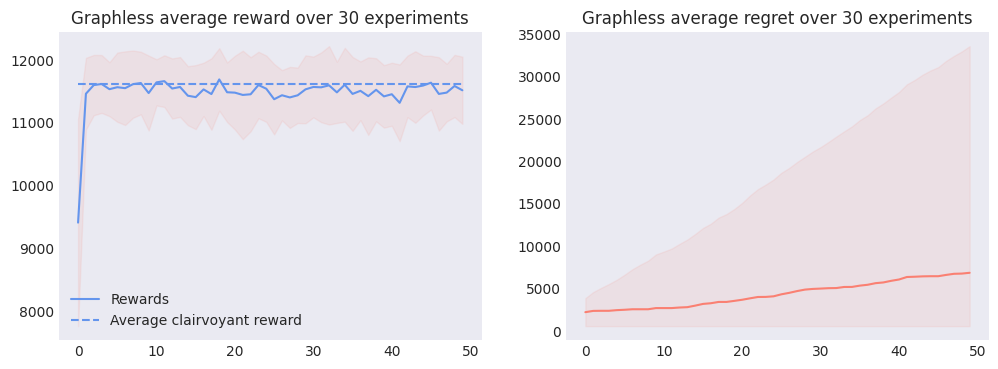
\includegraphics[scale=0.4]{img/Graphs/graphless/image2.png}
\end{center}

\vspace*{2em}

\scriptsize All tests are done using the \texttt{example\_environment} default values, \textit{population mean} of 1000, \textit{variance} of 10 and 20 \textit{budget steps}.

\end{frame}

% ----------------------------------------

\begin{frame}

\frametitle{Results}

We can observe that the regret is exceptionally low w.r.t the previous learners, this is most likely due to the fact that the \textbf{graphless learner} holds most of the important information from the environment and is able to give accurate estimations from the start.

However, some variance is always present due to the \textit{imperfect graph estimation} and \textit{environment non-determinism}.

Average results over 30 runs at time horizon $T = 50$:

\begin{table}
	\begin{tabular}{|c|cc|c|}
	\hline \hline
		\cellcolor{blue!25} & Reward 	& Regret	& Deviation \\
	\cline{2-4}
		\cellcolor{blue!25} & $\mu$		& $\mu$		& $\sigma$	\\
	\hline \hline
		Graphless			& 11515.87 	& 6845.87	& 534.97 	\\
	\hline \hline
	\end{tabular}
\end{table}

\end{frame}

% ----------------------------------------
